\documentclass[aspectratio=169]{beamer} % Set the document class as 'beamer'  in LaTeXwith an aspect ratio of 16:9.

%Make sure you use XeLaTeX as the compiler.

% Title page
	\title{Beamer Presentation Tutorial} % Title of the presentation.
	\subtitle{Learning by Example} % Subtitle for additional context.
	%\author{Michael Lotspeich-Yadao, Ph.D.\\\textit{\footnotesize{mlots2@illinois.edu}}} % Maybe you want a bigger name and email?
	\author{Michael Lotspeich-Yadao, Ph.D.} % Author name(s).
	\institute{For more resources, check out https://github.com/mlots2-illinois} % Institutional affiliation. I don't need this, so I commented it out.
	%\date{\today} % Date of the presentation.
	\date{} %If you leave it blank, it won't write the date on the title page.

% Theme and style selection
	\usetheme{Frankfurt} % Select the Frankfurt theme for a simple, modern layout.
	%I like this one because it includes the minipage navigation at the top of the screen.

% Package imports
	\usepackage{sourcesanspro} % Use Source Sans Pro font for a clean, modern look.
	\usepackage{booktabs} % For professional-looking tables with better spacing and lines.
	\usepackage{graphicx} % For including and manipulating images (scaling, rotating, etc.).
	\usepackage{amsmath}  % For advanced mathematical symbols and features (equations, matrices, etc.).
	\usepackage{graphicx} % Duplicate package, already included above. You can remove this.
	\usepackage{fontspec} % Allows use of custom system fonts (works with XeLaTeX or LuaLaTeX).
	\usepackage{xcolor} % For adding colors to text, tables, and other elements in your document.
	\usepackage{tikz} % For creating high-quality illustrations and diagrams.
		\usetikzlibrary{calc} % Add this line for performing coordinate calculations and other operations in TikZ.
	\usepackage{listings} % For including and formatting source code in various programming languages.
	\usepackage{lipsum} % For generating placeholder text (Lorem Ipsum).
	\usepackage{enumitem} % Provides better control over list formatting (itemize, enumerate, etc.).

% Font configuration
	% Define the primary and secondary fonts used throughout the presentation, based
	% on the institutional brand book.
	\setsansfont{Source Sans Pro}[Weight=300] % Sets Source Sans Pro Light as the default font.
	\newfontfamily\MontserratBold{Montserrat}[Weight=700] % Defines Montserrat Bold for headings.
	\newfontfamily\MontserratMedium{Montserrat}[Weight=500] % Defines Montserrat Medium for subtitles.
	% Beamer font customization
	% Specify how fonts appear in different contexts within the Beamer presentation.
		%\setbeamerfont{frametitle}{family=\MontserratBold, size=\Large} % Frame titles in Montserrat Bold.
		%\setbeamerfont{framesubtitle}{family=\MontserratMedium, size=\normalsize} % Subtitles in Montserrat Medium.
		\setbeamerfont{normal text}{family=\sffamily} % Normal text in Source Sans Pro.

% Navigation symbols removal
	% Remove the default navigation symbols (arrows, home, etc.) for a cleaner look.
	\setbeamertemplate{navigation symbols}{}

% Institutional color scheme
	% Define custom colors based on institutional branding.
		\definecolor{IlliniOrange}{cmyk}{0,0.8,1,0}
		\definecolor{Altgeld}{cmyk}{0,0.68,0.91,0.22}
		\definecolor{IlliniBlue}{cmyk}{1,0.90,0.10,0.50}
		\definecolor{IlliniStorm}{cmyk}{0.30,0.20,0.19,0}
		% Storm can be used to help obey a table in a design piece.
		
		% Supporting colors. If needed, can be reused at a tint of 20, 40, 60, 80%.
		\definecolor{industrial}{cmyk}{0.90,0.48,0,0}
		\definecolor{patina}{cmyk}{0.93,0.34,0.39,0.05}
		\definecolor{harvest}{cmyk}{0,0.20,0.60,0}
		\definecolor{earth}{cmyk}{0.33,0.76,1.00,0.36}
		\definecolor{arches}{cmyk}{0.70,0.05,0.02,0}
		\definecolor{berry}{cmyk}{0.53,1,0.42,0.43}
		\definecolor{prairie}{cmyk}{1,0.13,1,0.44}
		
		\definecolor{IlliniGray1}{cmyk}{0.18,0.12,0.11,0.35}
		\definecolor{IlliniGray2}{cmyk}{0.07,0.05,0.05,0.14}
		\definecolor{IlliniWhite}{cmyk}{0,0,0,0}
	
	\setbeamercolor{structure}{fg=blue!20!black}
	\beamertemplateshadingbackground{purple!0}{white}

% Begin document
\begin{document}
	
%Create the title slide	
	\begin{frame}
		~\\
		\center{
\includegraphics[width=1.25cm]{{University Graphics/Illinois_logo_fullcolor_rgb.eps}}} % Center the logo (image from file path).
		\\
		\titlepage % Automatically generates the title slide using the \title, \author, and \date information.
	\end{frame}
	
	% Create a frame for the table of contents
	\begin{frame}
		\tableofcontents % Automatically generates the table of contents based on sections and subsections.
	\end{frame}
	
\section{What is Beamer?} %Define a new section called "What is Beamer?"
	
	% Frame with a title and subtitle
	\begin{frame}{What is Beamer?} % Set frame title as "What is Beamer?"
		\framesubtitle{Overview} % Set subtitle for the frame.
		Beamer is a LaTeX class used for creating professional presentations. It allows users to:
		\begin{itemize}[label=\textbullet] % Creates a bullet point list with custom bullet symbol.
			\item Organize content into frames and sections.
			\item Use mathematical typesetting.
			\item Incorporate images, tables, and multimedia.
			\item Customize themes and layouts.
		\end{itemize}
	\end{frame}
	
	% Frame with title and subtitle
	\begin{frame}{I'm a frame title!} % Set frame title.
		\framesubtitle{I'm a subtitle!} % Set subtitle for the frame.
		But if you choose to, you can omit both the title and subtitle. To customize the banner at the top, use the \texttt{/section} command. % Example of not including a title or subtitle.
	\end{frame}
	
	% Frame with a title and bullet list
	\begin{frame}
		\frametitle{Basic Structure of a Beamer Presentation} % Set the frame title.
		A basic Beamer presentation consists of:
			\begin{itemize}[label=\textbullet] % Creates a bullet point list.
				\item Title page % Add a bullet point for the title page.
				\item Sections and frames % Add a bullet point for sections and frames.
				\item Overlay commands % Add a bullet point for overlay commands.
			\end{itemize}
	\end{frame}
	
	\begin{frame}
		\frametitle{Text and Font Styles} % Frame title.
		You can change the font style using the following commands:
			\begin{itemize} [label=\textbullet] % Creates a bullet point list.
				\item \textbf{Bold} % Bold text.
				\item \textit{Italic} % Italic text.
				\item \underline{Underlined} % Underlined text.
				\item \texttt{Typewriter font} % Typewriter-style font (monospaced).
			\end{itemize}
	\end{frame}
	
	%Color usage
	\begin{frame}
		\frametitle{Using Colors} % Frame title.
		You can use color for text, blocks, and items:
		 \texttt{\textcolor{red}{Red text}} and \texttt{\textcolor{blue}{Blue text}}. % Display text in different colors.
		 ~\\~\\
		Here is a colored block, how neat!
			\begin{block}{Colored Block} % Creates a block with a title.
    				This block uses custom colors.
  			\end{block}
	\end{frame}
	
	%More fancy colors
	\begin{frame}
		\frametitle{Blocks and Alerts} % Frame title.
		 You can create alerts or blocks for important information:
		 
		 \begin{alertblock}{Important} % Creates an alert block with a title "Important".
			This is an important note. % Content inside the alert block.
			\end{alertblock} % End of alert block.
  
		\begin{exampleblock}{Example} % Creates an example block with a title "Example".
			This is an example block. % Content inside the example block.
			\end{exampleblock} % End of example block.
  
	\end{frame}
	
	% Lists
	\begin{frame}
		\frametitle{Lists} % Frame title.
		You can create itemized lists:
		\begin{itemize}[label=\textbullet]  % Creates a bullet point list.
			\item Item 1 % First bullet point.
			\item Item 2 % Second bullet point.
		\end{itemize}
		~\\~\\
  		Or an enumerated list:
			\begin{enumerate} [label=\arabic*.]% Creates a numbered list.
				\item First item % First numbered item.
				\item Second item % Second numbered item.
			\end{enumerate}
	\end{frame}

	

	
\section{Do you use iClicker?}

\begin{frame}{iClicker Question}
	\setbeamerfont{itemize/enumerate body}{size=\large} %This makes the text bigger.
	\setbeamerfont{item projected}{size=\large} %This makes the bullet bigger.
	
	\begin{tikzpicture}[remember picture, overlay]
		\node[anchor=north east, yshift=-0.55cm] at (current page.north east) {
		 
\includegraphics[width=1.5cm]{iclicker.png} };
	\end{tikzpicture}

	\textbf{Which of the following best illustrates how the concept of \textit{social constructivism} is applied to understanding societal norms and values?}\\
	\begin{enumerate}[label=\Alph*.]
	\item Social norms are biologically encoded and evolve over time based on genetic predispositions.
	\item Social values emerge from a consensus among individuals within a society, reflecting shared meanings and agreements.
	\item Power dynamics between dominant and subordinate groups shape norms through coercion and exploitation.
	\item Institutions such as education and religion function to maintain societal stability by reinforcing pre-existing values.
	\item Individual behavior is determined by structural forces that operate independently of human agency.
	\end{enumerate}

\end{frame}
	
	
	
\section{More things that you can do}
	
	\subsection{Computer code}
	
	\begin{frame}[fragile]{Stata Code Example}% [fragile] allows for verbatim-like environments.
	Here is an example of a simple Stata script:
\begin{lstlisting}
use dataset.dta, clear
generate age_squared = age^2
regress income age age_squared
summarize income age age_squared
\end{lstlisting}

	\end{frame}
	
	\subsection{Images}
	
	\begin{frame}{Full-Page Image}
		\center{ \includegraphics[height=7cm, keepaspectratio]{University Photography/campus_photo5.jpg}}
	\end{frame}
	
	\begin{frame}{Half-Page Image and Text}
		\begin{columns}
			\column{0.5\textwidth}
			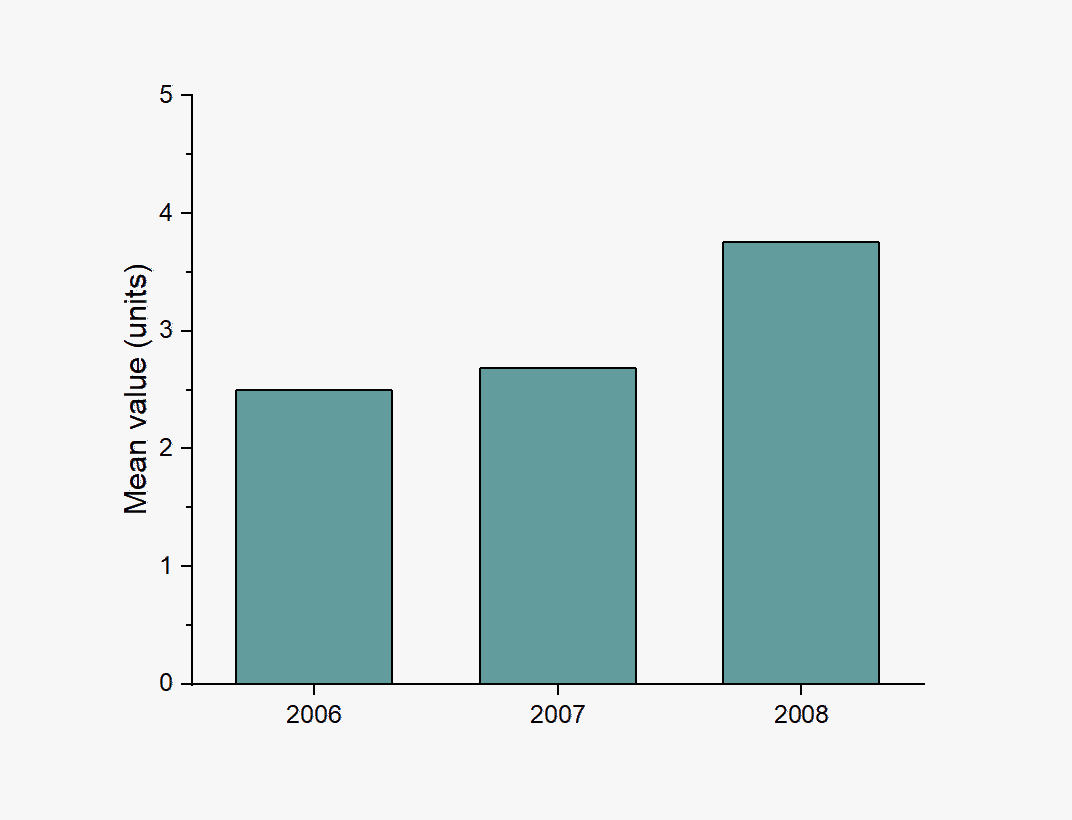
\includegraphics[width=\textwidth]{generic_bargraph.png}
			\column{0.5\textwidth}
			Beamer makes it simple to combine images and text. You can adjust the proportions of each column to suit your content.
		\end{columns}
	\end{frame}

	\begin{frame}{Half-Page Image and Text (flipped)}
		\begin{columns}
			\column{0.5\textwidth}
			You can also flip items around by rearranging the items on the slide. How neat!
			\column{0.5\textwidth}
			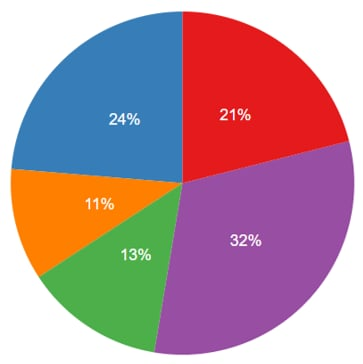
\includegraphics[width=\textwidth]{generic_piechart.png}
		\end{columns}
	\end{frame}
	
	
	\subsection{Equations}
	
\begin{frame}
\frametitle{Hill-Function based method}
\begin{equation*} \label{eq: main odes10-main1-last}
\frac{dr_a}{d\tau}=\frac{T_0}{H_r} \left(\left[1-\prod_{j=1}^{K_a}\rho(\alpha_{aj} r_{j},S_{aj}, k_{aj})\right]\prod_{m=K_a+1}^{J_a}\rho(\alpha_{am} r_{m},S_{am}, k_{am})-r_a(t)\right)\end{equation*}

\end{frame}
	
% Section: Columns and Tables
	\section{Columns and tables, too!}
	
	\begin{frame}{Columns Example}
		\begin{columns}
			\column{0.5\textwidth}
			\textbf{Column 1:} \\
			\begin{itemize}[label=\textbullet] 
				\item Point 1
				\item Point 2
				\item Point 3
			\end{itemize}
			\column{0.5\textwidth}
			\textbf{Column 2:} \\
			\begin{itemize}[label=\textbullet] 
				\item Another point
				\item Yet another point
			\end{itemize}
		\end{columns}
	\end{frame}
	
	\begin{frame}{Table Example}
		\begin{table}
			\centering
			\begin{tabular}{l c r}
				\toprule
				Item & Quantity & Price \\
				\midrule
				Apples & 5 & \$3.00 \\
				Bananas & 2 & \$1.50 \\
				Cherries & 10 & \$7.00 \\
				\bottomrule
			\end{tabular}
			\caption{A simple table.}
		\end{table}
	\end{frame}


\section{Variations on the title slide}
\begin{frame}
	If you don't like any of the title slides, or are looking for section slides, consider using some of these next slides!
\end{frame}

\begin{frame}[plain] %This example of a frame has a transparent polygon, background image, University-level logo, and a title for a section.

	% Background photo
	\begin{tikzpicture}[remember picture, overlay]
    		\node[anchor=south west, inner sep=0] at (current page.south west) {
        		\includegraphics[width=\paperwidth,height=\paperheight]{University Photography/campus_photo1.jpg}};
	\end{tikzpicture}
	
	% Diagonal polygon
	\begin{tikzpicture}[remember picture, overlay]
		\fill[IlliniBlue, opacity=0.9] (current page.south west) -- ([xshift=3cm]current page.south west) -- ([xshift=-3cm]current page.north east) --  (current page.north west) -- cycle;
	\end{tikzpicture}

	% Block I logo
	\begin{tikzpicture}[remember picture, overlay]
		\node[anchor=north west, xshift=0.5cm, yshift=-0.5cm] at (current page.north west) {
		
\includegraphics[width=1cm]{{University Graphics/Illinois_logo_reversed_orange_rgb.eps}}};
	\end{tikzpicture}
	
	%Section title
	\begin{tikzpicture}[remember picture, overlay] 
		\node[anchor=west, xshift=-7.5cm] at ([yshift=0.5cm]current page.center) 
		{\textcolor{white}{\Large \textbf{Your Title Here}}};
	\end{tikzpicture}

	%Section subtitle
	\begin{tikzpicture}[remember picture, overlay]
		\node[anchor=west, xshift=-7.5cm] at ([yshift=-0.25cm]current page.center) {
		\textcolor{white}{\normalsize \textit{Your Subtitle Here}}};
	\end{tikzpicture}

\end{frame}
	

\begin{frame}[plain] %If you choose not to use the Block I logo, then you can use a college-level logo

	% Background photo
	\begin{tikzpicture}[remember picture, overlay]
    		\node[anchor=south west, inner sep=0] at (current page.south west) {
        		\includegraphics[width=\paperwidth,height=\paperheight]{University Photography/campus_photo3.jpg}};
	\end{tikzpicture}
	
	% Diagonal polygon
	\begin{tikzpicture}[remember picture, overlay]
		\fill[IlliniBlue, opacity=0.9] (current page.south west) -- ([xshift=3cm]current page.south west) -- ([xshift=-3cm]current page.north east) --  (current page.north west) -- cycle;
	\end{tikzpicture}

	%If you choose not to use the Block I logo, then you can use a college-level logo
	\begin{tikzpicture}[remember picture, overlay]
		\node[anchor=north west, xshift=-0.2cm, yshift=0.1cm] at (current page.north west) {
		
\includegraphics[width=8cm]{{University Graphics/Primary_Unit_Wordmarks_Reversed_Orange_RGB_Grainger-Engineering.eps}}};	
	\end{tikzpicture}
	
	%Section title
	\begin{tikzpicture}[remember picture, overlay] 
		\node[anchor=west, xshift=-7.5cm] at ([yshift=0.5cm]current page.center) 
		{\textcolor{white}{\Large \textbf{Your Title Here}}};
	\end{tikzpicture}

	%Section subtitle
	\begin{tikzpicture}[remember picture, overlay]
		\node[anchor=west, xshift=-7.5cm] at ([yshift=-0.25cm]current page.center) {
		\textcolor{white}{\normalsize \textit{Your Subtitle Here}}};
	\end{tikzpicture}

\end{frame}
	
	
\begin{frame}[plain] %If you choose not to use the Block I logo, then you can use a college-level logo

	% Background photo
	\begin{tikzpicture}[remember picture, overlay]
    		\node[anchor=south west, inner sep=0] at (current page.south west) {
        		\includegraphics[width=\paperwidth,height=\paperheight]{University Photography/campus_photo5.jpg}};
	\end{tikzpicture}
	
	% Diagonal polygon
	\begin{tikzpicture}[remember picture, overlay]
		\fill[IlliniBlue, opacity=0.9] (current page.north west) -- ([xshift=3cm]current page.north west) -- ([xshift=-3cm]current page.south east) --  (current page.south west) -- cycle;
	\end{tikzpicture}

	%If you choose not to use the Block I logo, then you can use a college-level logo
	\begin{tikzpicture}[remember picture, overlay]
		\node[anchor=north west, xshift=-0.2cm, yshift=-6cm] at (current page.north west) {
		
\includegraphics[width=8cm]{{University Graphics/Primary_Unit_Wordmarks_Reversed_Orange_RGB_LAS.eps}}};
	\end{tikzpicture}
	
	%Section title
	\begin{tikzpicture}[remember picture, overlay] 
		\node[anchor=west, xshift=-7.5cm] at ([yshift=0.5cm]current page.center) 
		{\textcolor{white}{\Large \textbf{Your Title Here}}};
	\end{tikzpicture}

	%Section subtitle
	\begin{tikzpicture}[remember picture, overlay]
		\node[anchor=west, xshift=-7.5cm] at ([yshift=-0.25cm]current page.center) {
		\textcolor{white}{\normalsize \textit{Your Subtitle Here}}};
	\end{tikzpicture}

\end{frame}
	
	
\begin{frame}[plain] %If you choose not to use the Block I logo, then you can use a college-level logo
	
	% Diagonal polygon
	\begin{tikzpicture}[remember picture, overlay]
		\fill[IlliniBlue, opacity=0.9] (current page.north east) -- ([xshift=-3cm]current page.north east) -- ([xshift=3cm]current page.south west) -- (current page.south east) -- cycle;
	\end{tikzpicture}
	
	%If you choose not to use the Block I logo, then you can use a college-level logo
	\begin{tikzpicture}[remember picture, overlay]
		\node[anchor=north west, xshift=7cm, yshift=-6cm] at (current page.north west) {
		
\includegraphics[width=8cm]{{University Graphics/IL_Nickname_Unit_Wordmarks_Reversed_Orange_RGB_ACES.eps}}};
	\end{tikzpicture}
	
	%Section title
	\begin{tikzpicture}[remember picture, overlay] 
		\node[anchor=west, xshift=-7.5cm] at ([yshift=0.5cm]current page.center) 
		{\textcolor{black}{\Large \textbf{Your Title Here}}};
	\end{tikzpicture}

	%Section subtitle
	\begin{tikzpicture}[remember picture, overlay]
		\node[anchor=west, xshift=-7.5cm] at ([yshift=-0.25cm]current page.center) {
		\textcolor{black}{\normalsize \textit{Your Subtitle Here}}};
	\end{tikzpicture}

\end{frame}

\begin{frame}{Conclusion}
  This concludes our Introduction to Beamer in LaTeX. You can create professional presentations with ease by utilizing these features.
\end{frame}

\end{document}
